\chapter{Постановка задачи}
\label{cha:analysis}
%
% % В начале раздела  можно напомнить его цель
%

Перед началом научно-исследовательской работы был проанализирован ряд статей, посвященных применению методов глубокого обучения для таких жанров игр, как FPS (шутеры от первого лица) \cite{bergdahl2020augmenting}, прятки \cite{baker2019emergent}, а также аркадные и гоночные игры \cite{tufano2022using}.

\section{Среда}

В качестве среды для работы была выбрана платформа \textit{Gym} на языке Python \cite{Gym} по следующим причинам:
\begin{itemize}
	\item[--] в \textit{Gym} представлен ряд встроенных игр, которые можно использовать для тестирования моделей;
	\item[--] \textit{Gym} выступает в качестве посредника между игровой средой и агентом (моделью), выполняя нужные команды и собирая информацию о состоянии среды на каждом шаге.
\end{itemize}

Среди игровых сред, входящих в \textit{Gym}, была выбрана Lunar Lander v2 \cite{lunarlanderv2}. В ней игроку или агенту предлагается посадить лунный лендер (посадочный модуль) на заданную площадку, обозначенную флагами. Игра начинается с того, что центру масс модуля, находящегося наверху экрана, сообщается случайная сила. На каждом моменте времени можно привести в действие один трех двигателей: левый, правый или основной, либо ничего не делать. Игровой эпизод заканчивается, если лендер совершает посадку или покидает область видимости.

\section{Архитектура}

В научной литературе, прочитанной в рамках исследовательской работы, наиболее часто используемым алгоритмом являлся Deep Q-Network (DQN). Задача данного алгоритма "--- формирование функции полезности \(Q\), заданную следующим уравнением Беллмана: \[Q(s_t, a_t) \leftarrow Q(s_t, a_t) + \alpha \cdot (r(s_t, a_t) + \gamma \cdot \max_a Q(s_{t+1}, a) - Q(s_t, a_t)),\] где 
\begin{itemize}
	\item[--] \(s_t\) "--- состояние среды в момент времени \(t\); 
	\item[--]  \(a_t\) "--- действие агента, совершенное в момент времени \(t\);
	\item[--] \(r(s_t, a_t)\) "--- награда, полученная при переходе из состояния \(s_t\) в состояние \(s_{t+1}\);
	\item[--] \(\alpha \in (0, 1]\) "--- скорость обучения;
	\item[--] \(\gamma \in [0, 1]\) "--- дисконтирующий множитель; чем ближе он к единице, тем больше моделью будет учитываться награда в последующих состояниях.
\end{itemize}

Исследование агентом новых состояний и действий происходит благодаря $\varepsilon$-жадной стратегии принятия решений. Все они записываются в буфер воспроизведения (replay buffer), откуда на каждом шаге случайным образом выбирается партия из \(n\) кортежей вида \((s_t, a_t, r(s_t, a_t), s_{t+1})\).

В DQN используются две нейросети: одна отвечает за оценку \(Q\) для текущего состояния и обновляется на каждом шаге, когда как другая вычисляет оптимальное значения \(Q\) для последующего состояния (её веса изменяются периодически).

В качестве функции потерь была выбрана функция Хьюбера, т.~к. она является менее чувствительной к выбросам, нежели среднеквадратическая ошибка (MSE).

Для достижения большей стабильности при обучении использовалась модификация стандартного алгоритма DQN, называемая Dueling Double Deep Q-Network (D3QN) \cite{wang2016dueling,hasselt2016deep}. Кривая обучения такой модели представлена на рис.~\ref{fig:trainScore}

\begin{figure}
	\centering
	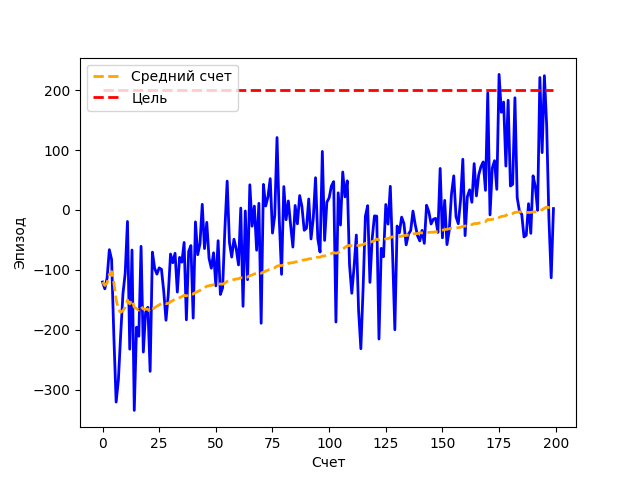
\includegraphics[width=\textwidth]{figures/d3qn_train_score}
	\caption{Пример кривой обучения D3QN в среде Lunar Lander v2.}
	\label{fig:trainScore}
\end{figure}

%Кстати, про картинки. Во-первых, для фигур следует использовать \texttt{[ht]}. Если и после этого картинки вставляются <<не по ГОСТ>>, т.е. слишком далеко от места ссылки, "--- значит у вас в РПЗ \textbf{слишком мало текста}! Хотя и ужасный параметр \texttt{!ht} у окружения \texttt{figure} тоже никто не отменял, только при его использовании документ получается страшный, как в ворде, поэтому просьба так не делать по возможности.

%\begin{enumerate}
%\item Перечисление с номерами.
%\item Номера первого уровня. Да, ГОСТ требует именно так "--- сначала буквы, на втором уровне "--- цифры.
%Чуть ниже будет вариант <<нормальной>> нумерации и советы по её изменению.
%Да, мне так нравится: на первом уровне выравнивание элементов как у обычных абзацев. Проверим теперь вложенные списки.
%\begin{enumerate}
%\item Номера второго уровня.
%\item Номера второго уровня. Проверяем на длииииной-предлиииииииииинной строке, что получается.... Сойдёт.
%\end{enumerate}
%\item По мнению Лукьяненко, человеческий мозг старается подвести любую проблему к выбору
%  из трех вариантов.
%\item Четвёртый (и последний) элемент списка.
%\end{enumerate}
%
%Теперь мы покажем, как изменить нумерацию на «нормальную», если вам этого захочется. Пара команд в начале документа поможет нам.
%
%\renewcommand{\labelenumi}{\arabic{enumi})}
%\renewcommand{\labelenumii}{\asbuk{enumii})}
%
%\begin{enumerate}
%\item Изменим нумерацию на более привычную...
%\item ... нарушим этим гост.
%\begin{enumerate}
%\item Но, пожалуй, так лучше.
%\end{enumerate}
%\end{enumerate}
%
%В заключение покажем произвольные маркеры в списках. Для них нужен пакет \textbf{enumerate}.
%\begin{enumerate}[1.]
%\item Маркер с арабской цифрой и с точкой.
%\item Маркер с арабской цифрой и с точкой.
%\begin{enumerate}[I.]
%\item Римская цифра с точкой.
%\item Римская цифра с точкой.
%\end{enumerate}
%\end{enumerate}
%
%В отчётах могут быть и таблицы "--- см. табл.~\ref{tab:tabular} и~\ref{tab:longtable}.
%Небольшая таблица делается при помощи \Code{tabular} внутри \Code{table} (последний
%полностью аналогичен \Code{figure}, но добавляет другую подпись).
%
%\begin{table}[ht]
%  \caption{Пример короткой таблицы с коротким названием}
%  \begin{tabular}{|r|c|c|c|l|}
%  \hline
%  Тело      & $F$ & $V$  & $E$ & $F+V-E-2$ \\
%  \hline
%  Тетраэдр  & 4   & 4    & 6   & 0         \\
%  Куб       & 6   & 8    & 12  & 0         \\
%  Октаэдр   & 8   & 6    & 12  & 0         \\
%  Додекаэдр & 20  & 12   & 30  & 0         \\
%  Икосаэдр  & 12  & 20   & 30  & 0         \\
%  \hline
%  Эйлер     & 666 & 9000 & 42  & $+\infty$ \\
%  \hline
%  \end{tabular}
%  \label{tab:tabular}
%\end{table}
%
%Для больших таблиц следует использовать пакет \Code{longtable}, позволяющий создавать
%таблицы на несколько страниц по ГОСТ.
%
%Для того, чтобы длинный текст разбивался на много строк в пределах одной ячейки, надо в
%качестве ее формата задавать \texttt{p} и указывать явно ширину: в мм/дюймах
%(\texttt{110mm}), относительно ширины страницы (\texttt{0.22\textbackslash textwidth})
%и~т.п.
%
%Можно также использовать уменьшенный шрифт "--- но, пожалуйста, тогда уж во \textbf{всей}
%таблице сразу.
%
%\begin{center}
%  \begin{longtable}{|p{0.40\textwidth}|c|p{0.30\textwidth}|}
%    \caption{Пример длинной таблицы с длинным названием на много длинных-длинных строк}
%    \label{tab:longtable}
%    \\ \hline
%    Вид шума & Громкость, дБ & Комментарий \\
%    \hline \endfirsthead
%    \subcaption{Продолжение таблицы~\ref{tab:longtable}}
%    \\ \hline \endhead
%    \hline \subcaption{Продолжение на след. стр.}
%    \endfoot
%    \hline \endlastfoot
%    Порог слышимости             & 0     &                                                \\
%    \hline
%    Шепот в тихой библиотеке     & 30    &                                                \\
%    Обычный разговор             & 60-70 &                                                \\
%    Звонок телефона              & 80    & \small{Конечно, это было до эпохи мобильников} \\
%    Уличный шум                  & 85    & \small{(внутри машины)}                        \\
%    Гудок поезда                 & 90    &                                                \\
%    Шум электрички               & 95    &                                                \\
%    \hline
%    Порог здоровой нормы         & 90-95 & \small{Длительное пребывание на более
%    громком шуме может привести к ухудшению слуха}                                        \\
%    \hline
%    Мотоцикл                     & 100   &                                                \\
%    Power Mower                  & 107   & \small{(модель бензокосилки)}                  \\
%    Бензопила                    & 110   & \small{(Doom в целом вреден для здоровья)}     \\
%    Рок-концерт                  & 115   &                                                \\
%    \hline
%    Порог боли                   & 125   & \small{feel the pain}                          \\
%    \hline
%    Клепальный молоток           & 125   & \small{(автор сам не знает, что это)}          \\
%    \hline
%    Порог опасности              & 140   & \small{Даже кратковременное пребывание на
%    шуме большего уровня может привести к необратимым последствиям}                       \\
%    \hline
%    Реактивный двигатель         & 140   &                                                \\
%                                 & 180   & \small{Необратимое полное повреждение
%                                 слуховых органов}                                        \\
%    Самый громкий возможный звук & 194   & \small{Интересно, почему?..}                   \\
%  \end{longtable}
%\end{center}

%%% Local Variables:
%%% mode: latex
%%% TeX-master: "rpz"
%%% End:
